\newpage
\section{Numérisation}
Beaucoup de phénomènes physiques nécessitent un capteur quelconque pour pouvoir être mesurés et analysés par un ordinateur. Dans le cas du son, un micro capte les variations de la pression d'air afin de convertir l'onde sonore en un signal électrique la représentant. Alors, on dit qu'il s'agit d'un signal analogique, car il est analogue aux variations de la pression d'air. Tout de même, le signal qui en découle reste continu et il doit être numérisé afin qu'un ordinateur puisse s'en servir. Cette numérisation en demande l'échantillonnage, la quantification et l'encodage.

\subsection{Échantillonnage}
L'échantillonnage correspond à l'action de discrétiser dans le temps un signal analogique entrant. Étant continu, il est impossible de l'enregistrer dans son entièreté, à chaque instant précis, en mémoire sur un ordinateur. Autrement, il faudrait une quantité infinie de mémoire et faire l'analyse de toutes ces données serait un enfer. Alors, on prend des mesures à intervalles réguliers (des échantillons) afin de construire une représentation discrète du signal électrique.

\begin{figure}[H]
    \centering
        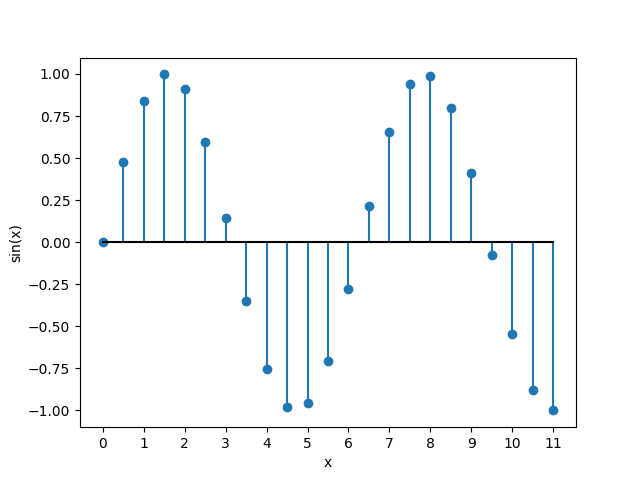
\includegraphics[width=0.5\textwidth]{images/ch6/echantillonage.png}
    \caption{Exemple d'échantillonnage de $\sin(x)$}
    \label{fig_ech_sin}
    \end{figure}

Le rythme auquel on décide de prendre les mesures se nomme la fréquence d'échantillonnage $f_s = \frac{1}{\Delta t}$ où $\Delta t$ est le temps séparant chaque échantillon. Évidemment, plus la fréquence d'échantillonnage est grande, plus les mesures "ont l'air" du phénomène analogique qu'elles décrivent. Cependant, une trop grande fréquence d'échantillonnage donne beaucoup de points et leur traitement sera lent. Par ailleurs, une trop petite fréquence d'échantillonnage n'est peut-être pas suffisante pour obtenir une représentation fidèle du signal analogique. Ainsi, pour avoir toute l'information nécessaire avec le moins de données, quelle fréquence d'échantillonnage faut-il choisir?

\subsubsection{Repliement spectral (\textit{aliasing}) et théorème d'échantillonnage}
Soient deux signaux sinusoïdaux analogiques à une fréquence de 2Hz et 18Hz respectivement qu'on échantillonne à $f_s = 16$Hz. On s'aide du delta de Dirac comme pour la TFD.

\begin{equation*}
    \text{2Hz : } \sin(2\pi \cdot 2t) \xrightarrow{\text{échantillonnage}, \ f_s = 16 \text{Hz}} \sum_{m=-\infty}^{\infty}\sin(2\pi \cdot 2 \cdot \frac{m}{16}) \delta\left(t - \frac{m}{16}\right)
\end{equation*}
\begin{equation*}
    \text{18Hz : } \sin(2\pi \cdot 18t) \xrightarrow{\text{échantillonnage}, \ f_s = 16 \text{Hz}} \sum_{m=-\infty}^{\infty}\sin(2\pi \cdot 18 \cdot \frac{m}{16}) \delta\left(t - \frac{m}{16}\right)
\end{equation*}

\begin{figure}[H]
    \centering
        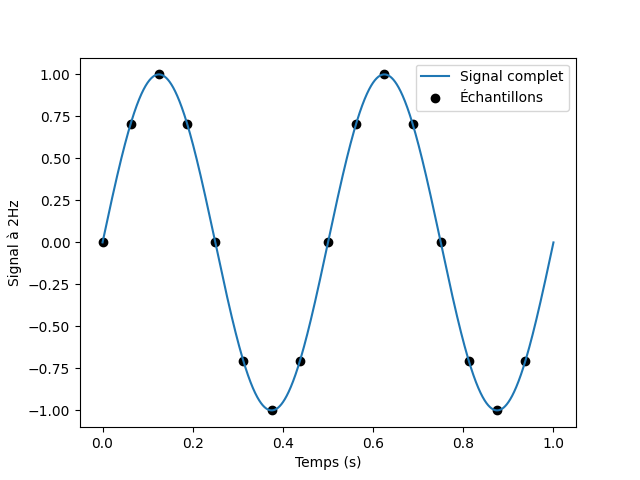
\includegraphics[width=0.48\textwidth]{images/ch6/2hz.png}
        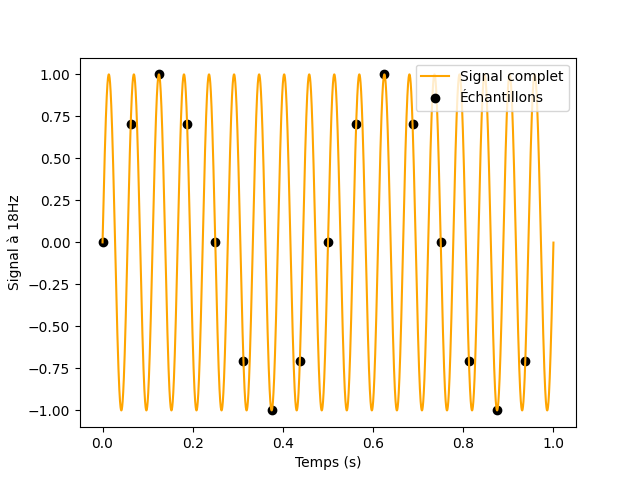
\includegraphics[width=0.48\textwidth]{images/ch6/18hz.png}
    \caption{Signal à 2Hz (à gauche) et signal à 18Hz (à droite) échantillonnés à $f_s = 16$Hz pour $t \in [0,1)$}
    \label{fig_2hz_18hz}
    \end{figure}

Si on superpose ces deux graphiques, on remarque que les échantillons des deux signaux sont exactement les mêmes.

\begin{figure}[H]
    \centering
        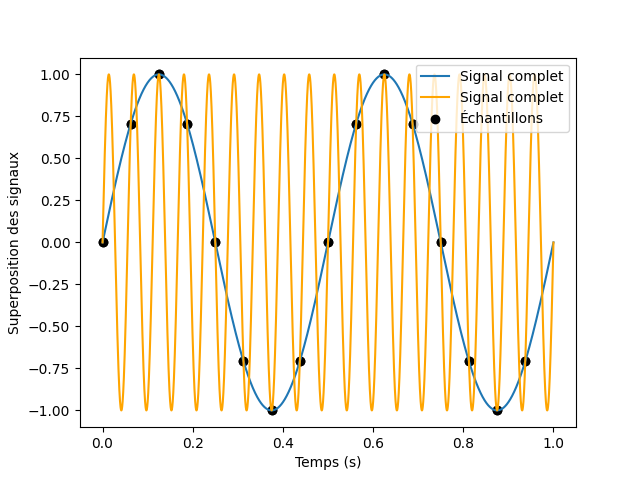
\includegraphics[width=0.48\textwidth]{images/ch6/superposition_2hz_18hz.png}
    \caption{Superposition des graphiques de la figure \ref{fig_2hz_18hz}}
    \label{fig_aliasing_2hz_18hz}
    \end{figure}

Cela est assez problématique, car depuis les échantillons mesurés à $f_s = 16$Hz, on ne peut pas distinguer s'il s'agit d'un signal à 2Hz ou à 18Hz. Une autre manière de le voir est de dire qu'à cette fréquence d'échantillonnage, le signal à 18Hz se comporte comme un signal à 2Hz tel un alias, d'où le nom \textit{aliasing}. En fait, avec un peu d'algèbre,

\begin{equation*}
    \sum_{m=-\infty}^{\infty}\sin(2\pi \cdot 18 \cdot \frac{m}{16}) \delta\left(t - \frac{m}{16}\right) = \sum_{m=-\infty}^{\infty}\sin(2\pi(2 + 1\cdot 16)\frac{m}{16}) \delta\left(t - \frac{m}{16}\right) 
\end{equation*}
\begin{equation*}
    = \sum_{m=-\infty}^{\infty}\sin(2\pi \cdot 2 \cdot \frac{m}{16} + 2\pi \cdot 1 \cdot m) \delta\left(t - \frac{m}{16}\right) = \sum_{m=-\infty}^{\infty}\sin(2\pi \cdot 2 \cdot \frac{m}{16})\delta\left(t - \frac{m}{16}\right)
\end{equation*}

et on voit mathématiquement l'\textit{aliasing}. De manière plus générale,

\begin{equation}
    \sum_{m=-\infty}^{\infty}\sin(2\pi f \frac{m}{f_s})\delta\left(t - \frac{m}{f_s}\right) = \sum_{m=-\infty}^{\infty}\sin(2\pi (f + lf_s)\frac{m}{f_s})\delta\left(t - \frac{m}{f_s}\right) \ \forall l \in \mathbb{Z}
    \label{eq_aliasing_sinus}
\end{equation}

et on peut ainsi calculer tous les alias possibles. Donc, dans l'exemple précédent, un signal de 34Hz sera aussi un alias du signal à 2Hz pour $f_s = 16$Hz. 

Quel est l'impact de l'échantillonnage sur le spectre de fréquence du signal à 2Hz? Normalement, après avoir appliqué la TF, on s'attend à uniquement deux pics à $\pm$2Hz. Cependant, à cause de l'échantillonnage, 

\begin{equation*}
    \text{TF}\left(\sum_{m=-\infty}^{\infty}\sin(2\pi \cdot 2 \cdot \frac{m}{16})\delta\left(t - \frac{m}{16}\right)\right) = \sum_{m=-\infty}^{\infty}\sin(2\pi \cdot 2 \cdot \frac{m}{16})e^{-i2\pi f\frac{m}{16}} \int_{-\infty}^{\infty}\delta\left(t - \frac{m}{16}\right)dt
\end{equation*}
\begin{equation*}
    = \sum_{m=-\infty}^{\infty}\sin(2\pi \cdot 2 \cdot \frac{m}{16})e^{-i2\pi f\frac{m}{16}} \cdot 1 = \sum_{m=-\infty}^{\infty}\sin(2\pi \cdot 2 \cdot \frac{m}{16})e^{-i2\pi f\frac{m}{16}} \cdot \text{TF}\left(\delta(t)\right) 
\end{equation*}
\begin{equation*}
    = \sum_{m=-\infty}^{\infty}\sin(2\pi \cdot 2 \cdot \frac{m}{16}) \cdot \text{TF}\left(\delta\left(t - \frac{m}{16}\right)\right) = \text{TF}\left(\sin(2\pi \cdot 2t)\sum_{m = -\infty}^{\infty}\delta\left(t - \frac{m}{16}\right)\right)
\end{equation*}
\begin{equation*}
    = \text{TF}\left(\sin(2\pi \cdot 2t)\cdot 16\sum_{m = -\infty}^{\infty}e^{i2\pi m\cdot 16t}\right) = 16\sum_{m=-\infty}^{\infty}\text{TF}\left(\sin(2\pi \cdot 2t) e^{i2\pi m\cdot 16t}\right)
\end{equation*}
\begin{equation*}
    = 16\sum_{m=-\infty}^{\infty}\text{TF}_{\text{déplacée par $16m$ sur l'axe des fréquences}}\left(\sin(2\pi \cdot 2t)\right)
\end{equation*}

où on a utilisé la propropriété de linéarité, de déplacement en temps et de déplacement en fréquences de la TF. Aussi, on utilise la série de Fourier du peigne de Dirac et la TF du delta de Dirac. On voit alors des copies de la TF du signal à 2Hz ($\pm 2$Hz) à chaque multiple de la fréquence d'échantillonnage $f_s = 16$, c'est-à-dire là où se trouvent les alias. 

\begin{figure}[H]
    \centering
        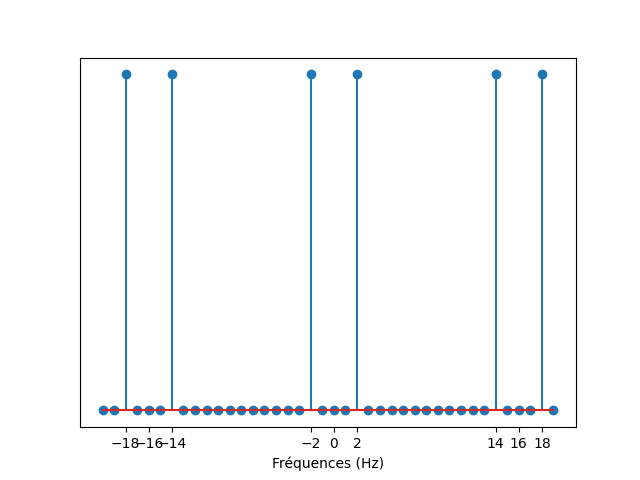
\includegraphics[width=0.48\textwidth]{images/ch6/aliasing_2hz.png}
    \caption{Effet de l'échantillonnage sur le spectre de fréquence du signal de 2Hz}
    \label{fig_copies_2hz}
    \end{figure}

Si la fréquence d'échantillonnage était plus grande, les copies deviendraient de plus en plus espacées et, dans la limite où $f_s$ est infini, on obtiendrait la véritable TF du signal à 2Hz avec uniquement les fréquences $\pm$2Hz. Cela a du sens, car en échantillonnant davantage, il y a de moins en moins d'alias possibles du fait qu'on représente mieux le signal.

Pour un signal échantillonné plus complexe ayant une plage limitée de fréquences entre $\pm f_{\text{max}}$, on voit ce même effet avec des copies plus ou moins espacées selon la fréquence d'échantillonnage (il suffit de généraliser la précédente dérivation).

\begin{equation}
    \text{TF}\left(\sum_{m=-\infty}^{\infty}f\left(\frac{m}{f_s}\right)\delta\left(t - \frac{m}{f_s}\right)\right) = f_s\sum_{m=-\infty}^{\infty}\text{TF}_{\text{déplacée par $f_sm$ sur l'axe des fréquences}}\left(f(t)\right)
    \label{eq_deplacement_freq_TF_echantillonage}
\end{equation}

\begin{figure}[H]
    \centering
        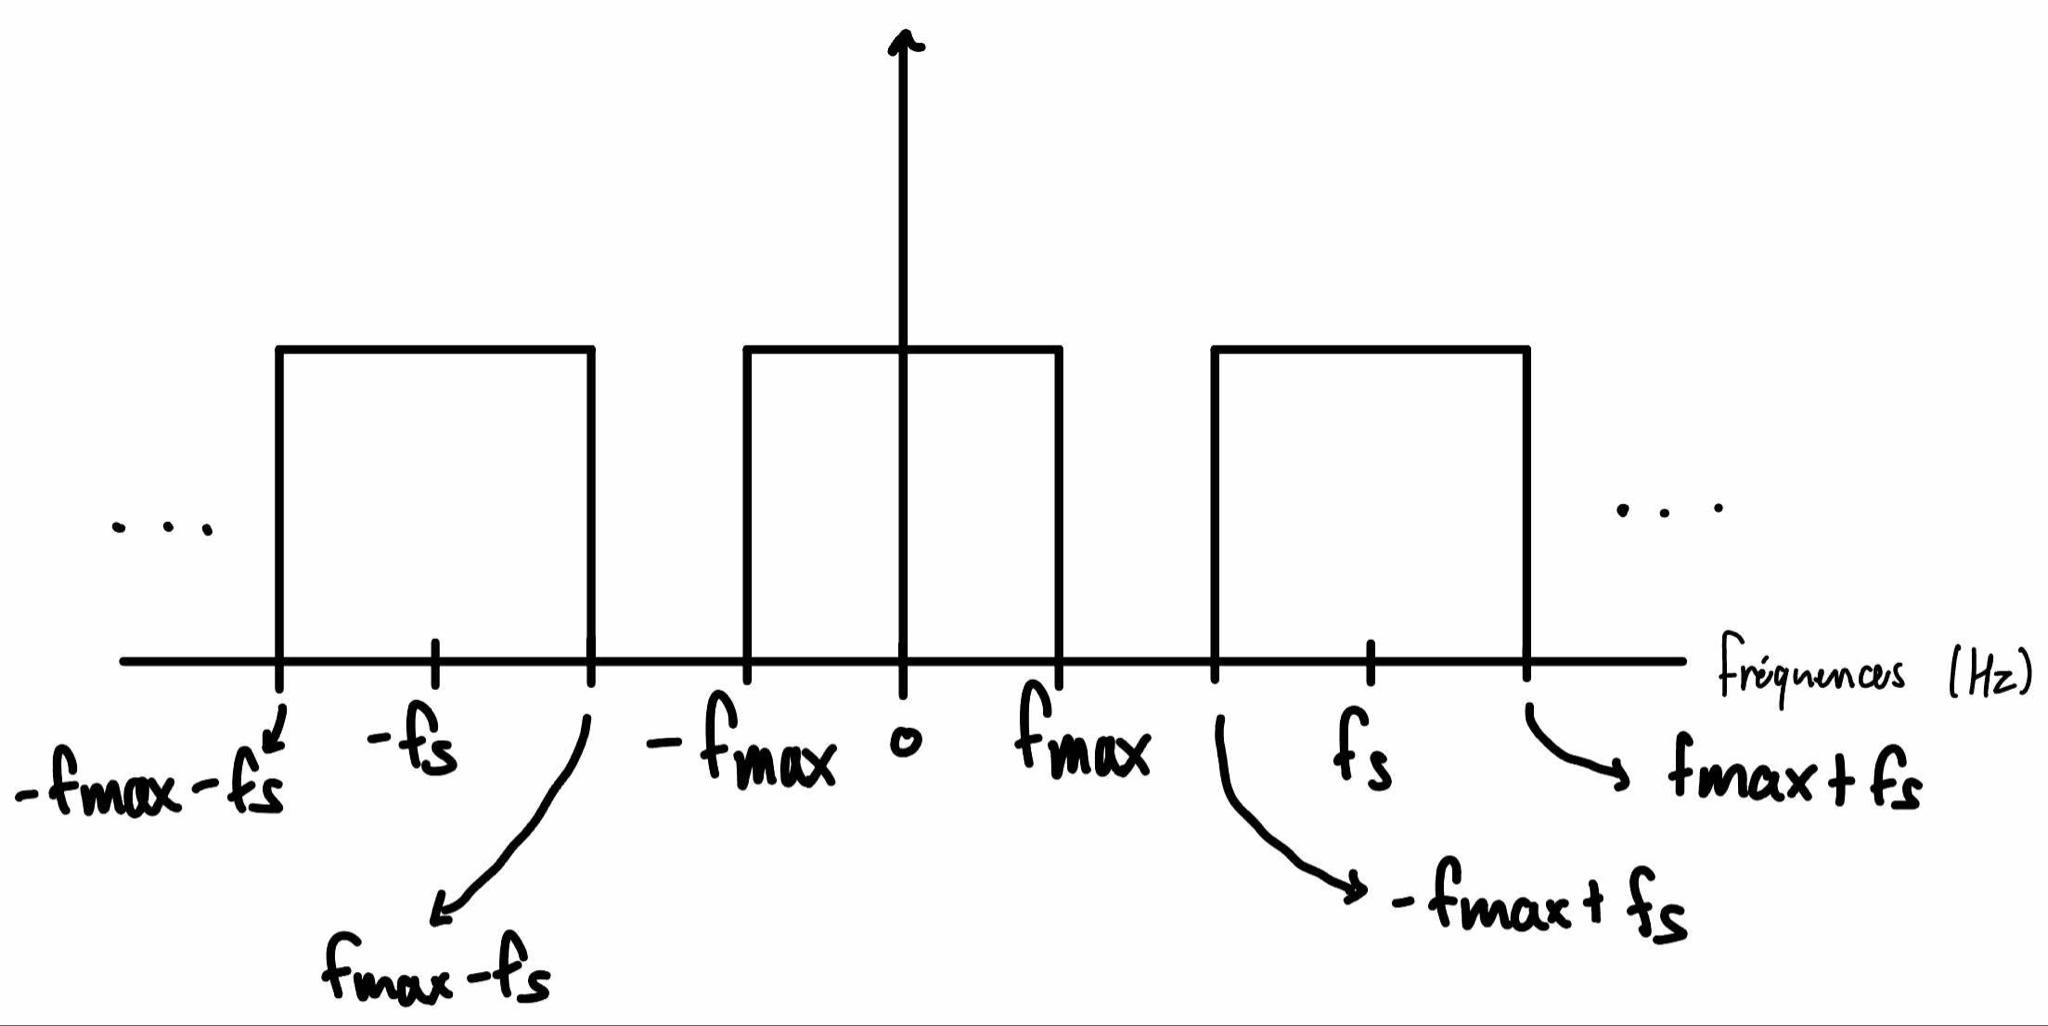
\includegraphics[width=0.6\textwidth]{images/ch6/aliasing_complexe.jpg}
    \caption{Effet de l'échantillonnage sur le spectre de fréquence d'un signal quelconque avec une plage de fréquences limitée}
    \label{fig_copies_xhz}
    \end{figure}

L'\textit{aliasing} semble être un problème seulement lorsqu'on ne sait pas la plage de fréquences que peut prendre un signal entrant. Autrement, si on sait que la plage de fréquences est $\pm f_{\text{max}}$, alors on regarde seulement là et ignore les copies au-delà. Cependant, si la fréquence d'échantillonnage est trop basse, les copies vont s'entremêler et le contenu fréquentiel sera altéré. En effet, le tout s'additionne et cela donnera l'impression qu'il y a davantage de certaines fréquences dans le signal par rapport à ce qu'on s'attendrait.  

\begin{figure}[H]
    \centering
        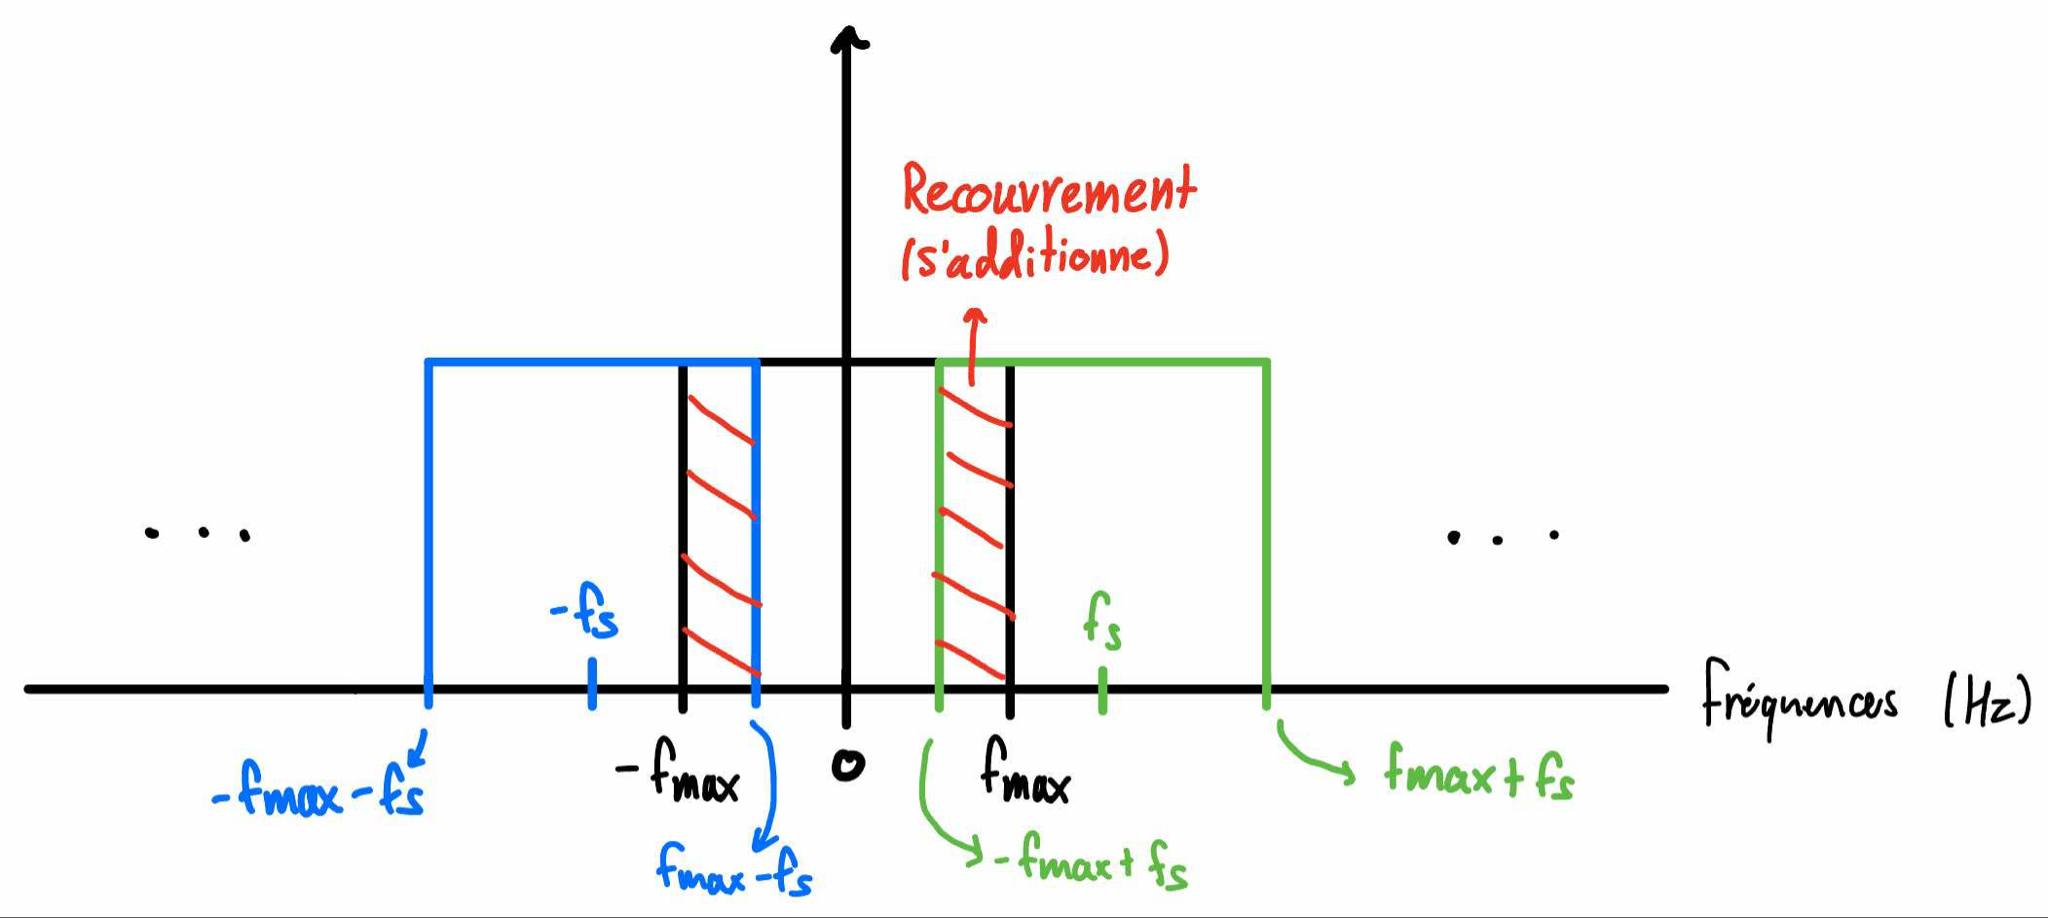
\includegraphics[width=0.7\textwidth]{images/ch6/aliasing_recouvrement.jpg}
    \caption{Effet de l'échantillonnage sur le spectre de fréquence d'un signal quelconque avec une plage de fréquences limitée quand la fréquence d'échantillonnage n'est pas assez grande}
    \label{fig_copies_recouvrement}
    \end{figure}

Pour éviter tout recouvrement, on voit par les précédentes figures qu'il est nécessaire que 

\begin{equation}
    f_s > 2f_{\text{max}}
    \label{eq_nyquist_shannon}
\end{equation}

C'est ce qu'on appelle le théorème d'échantillonnage et, si respecté, il garantit que l'\textit{aliasing} ne causera aucun problème et que l'échantillonnage représente fidèlement le signal original. De manière équivalente, on peut aussi dire que pour une fréquence d'échantillonnage $f_s$ donnée, la fréquence maximale qui ne subit pas les problèmes de l'\textit{aliasing} est $f_s / 2$ qu'on nomme la fréquence de Nyquist.

\subsubsection{Échantillonnage de l'audio}
Grosso modo, la plage de fréquences audibles pour les humains va de 20Hz à 20kHz. Donc, selon (\ref{eq_nyquist_shannon}), il faut que la fréquence d'échantillonnage d'un son soit supérieure à 40kHz. Par contre, en pratique, un micro va aussi enregistrer des fréquences bien au-delà de ce qu'on peut entendre et le choix de $f_s = 40$kHz ne sera pas suffisant pour éviter les problèmes dus à l'\textit{aliasing}. En fait, dans les convertisseurs analogique à numérique, qui font l'échantillonnage du son, il y a un filtre qui coupe les fréquences en dehors de la plage audible des humains. Pour des raisons techniques, le filtre ne peut pas couper nettement les fréquences pile au-delà de 20kHz et il restera quand même des fréquences, certes atténuées, un peu au-dessus de 20kHz. Alors, pour contrer l'\textit{aliasing}, on prend une fréquence d'échantillonnage un peu plus grande dont le standard est 44.1kHz, 48kHz et bien d'autres.  

\subsection{Quantification}
Pour le moment, on échantillone le signal en gardant son amplitude exacte car il s'agit d'un signal.



\subsection{Encodage}
